\section{Theoretical Results}
%
%
\begin{table}[h]
\centering
\caption{Properties of simulated clusters.
{\it Q: Einheit von $\Gamma$? 
Ich schlage vor, alle Zerfallsbreiten mit einem festen Exponenten von z.B. 10${-6}$ aufzuschreiben, und diesen wegzulassen. 
Es w\"urde dadurch sehr viel \"ubersichtlicher, und man sieht gleich welche Zerf\"alle \"uberhaupt wichtig sind.}
}
\begin{tabular}{lrrrccc}
\toprule
name                 & Xe atoms & Ar atoms & Xe \% &   ICD                &  ETMD                & $\Gamma_{\rm ICD,ETMD}$\\
\midrule
ArXe\_2\_1atom       &      1   &     12   &  7.7  &      0.0             &  0.0                 &     0.0            \\
ArXe\_3\_1atom       &      1   &     54   &  1.8  &      0.0             &  0.0                 &     0.0            \\ 
ArXe\_3\_2atom       &      2   &     53   &  3.6  & 3.346$\cdot 10^{-6}$ & 1.666$\cdot 10^{-5}$ & 2.006$\cdot 10^{-5}$ \\
ArXe\_8\_1layer      &   1415   &    642   & 68.8  & 7.039$\cdot 10^{-4}$ & 2.573$\cdot 10^{-4}$ & 9.612$\cdot 10^{-4}$ \\
\midrule
XeAr\_2\_surface     &      1   &     13   &  7.1  & 7.922$\cdot 10^{-5}$ & 0.0                  & 7.922$\cdot 10^{-5}$ \\
XeAr\_2\_edge        &      1   &     13   &  7.1  & 1.320$\cdot 10^{-6}$ & 0.0                  & 1.320$\cdot 10^{-6}$ \\
XeAr\_2\_vertex      &      1   &     13   &  7.1  & 5.013$\cdot 10^{-6}$ & 0.0                  & 5.013$\cdot 10^{-6}$ \\
XeAr\_2\_2top        &      2   &     13   & 13.3  & 1.011$\cdot 10^{-5}$ & 1.513$\cdot 10^{-5}$ & 2.523$\cdot 10^{-5}$ \\
XeAr\_2\_2midtop     &      2   &     13   & 13.3  & 1.588$\cdot 10^{-5}$ & 7.686$\cdot 10^{-7}$ & 1.665$\cdot 10^{-5}$ \\
XeAr\_2\_2endtop     &      2   &     13   & 13.3  & 1.587$\cdot 10^{-5}$ & 1.772$\cdot 10^{-7}$ & 1.605$\cdot 10^{-5}$ \\
XeAr\_3\_surface     &      1   &     55   &  1.8  & 6.371$\cdot 10^{-6}$ & 0.0                  & 6.371$\cdot 10^{-6}$ \\
XeAr\_3\_edge        &      1   &     55   &  1.8  & 4.791$\cdot 10^{-6}$ & 0.0                  & 4.791$\cdot 10^{-6}$ \\
XeAr\_3\_vertex      &      1   &     55   &  1.8  & 2.701$\cdot 10^{-6}$ & 0.0                  & 2.701$\cdot 10^{-6}$ \\
XeAr\_3\_edge\_in    &      1   &     54   &  1.8  & 7.708$\cdot 10^{-6}$ & 0.0                  & 7.708$\cdot 10^{-6}$ \\
XeAr\_3\_vertex\_in  &      1   &     54   &  1.8  & 5.258$\cdot 10^{-6}$ & 0.0                  & 5.258$\cdot 10^{-6}$ \\
XeAr\_3\_2in         &      2   &     53   &  3.6  & 1.166$\cdot 10^{-5}$ & 5.453$\cdot 10^{-6}$ & 1.711$\cdot 10^{-5}$ \\
XeAr\_3\_6in         &      6   &     49   & 10.9  & 3.746$\cdot 10^{-5}$ & 4.050$\cdot 10^{-5}$ & 7.796$\cdot 10^{-5}$ \\
XeAr\_3\_6\_scat     &      6   &     49   & 10.9  & 2.923$\cdot 10^{-5}$ & 6.737$\cdot 10^{-5}$ & 9.660$\cdot 10^{-5}$ \\
\bottomrule
\end{tabular}
\label{table:theo_gammas}
\end{table}
%
The geometrical properties as well as the total ICD and ETMD decay widths
of the investigated structures are shown in Table \ref{table:theo_gammas}.
It is important to remember that the first ICD channel opens at a
channel opening distance of \unit[7.58]{\AA}. Therefore, in small
clusters, in which none of the possible Ar-Xe pair distances is larger than
these \unit[7.58]{\AA}, no ICD can take place. Also, by definition two xenon atoms are
required for ETMD(3), hence it cannot occur in clusters with only one xenon atom.
%Because secondary electrons are observed in the experimental spectra
%we exclude all structures without any signal from our further
%discussions.
%
%In the investigated structures several different aspects have to be
%taken into account which we will discuss separately if possible
%on selected structures.

We will now discuss features of several structures, using selected examples.

Firstly, we consider two different argon core sizes one consisting
of 13 and one consisting of 55 atoms with one xenon atom on one of
the surfaces (see Figure \ref{figure:cluster_3_overview} Panel a)
for the 55 atom core). The simulated secondary electron spectra are
shown in Figure \ref{figure:surf} Panel 1.

\begin{figure}[ht]
 \centering
 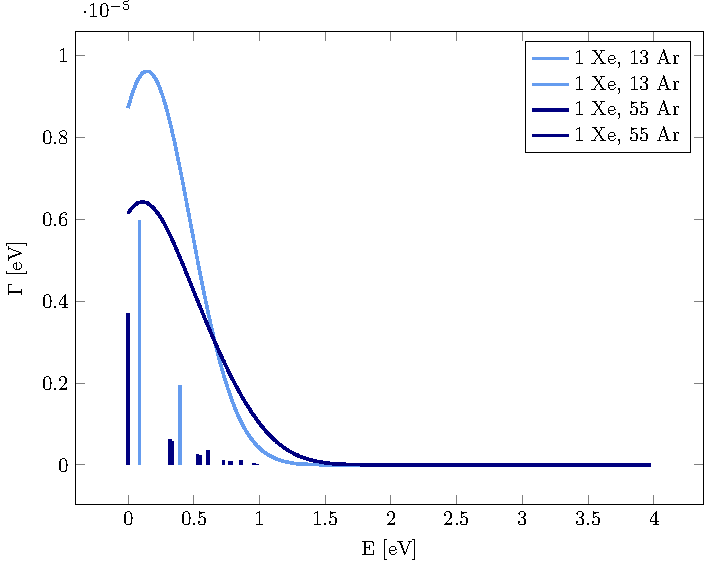
\includegraphics[width=8.5cm]{pics/surf.pdf}\\
 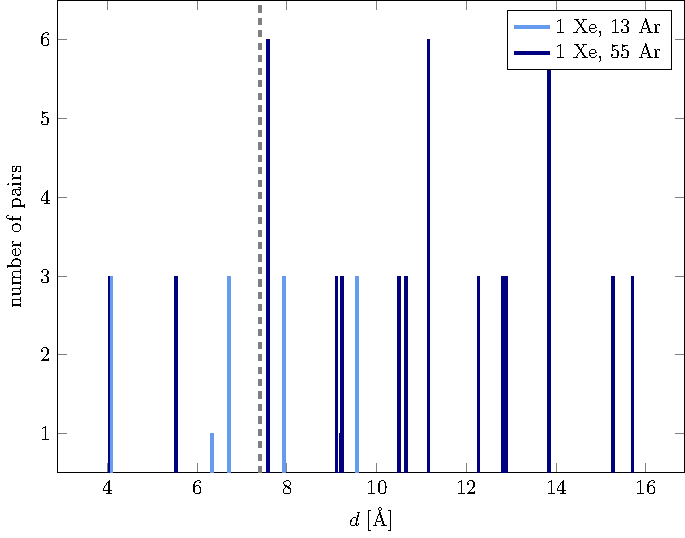
\includegraphics[width=8.2cm]{pics/R_comp.pdf}
 \caption{Panel 1: Simulated electron-electron coincidence spectra
          for argon clusters
          consisting of 13 and 55 atoms with on additional xenon atom residing
          on top of one of the argon surfaces.\\
          Panel 2: Distribution of Ar-Xe distances $d$ in the studied ArXe
          clusters. The ICD channels open at \unit[7.58]{\AA} and
          \unit[36.00]{\AA}, respectively. Hence only pairs at longer interatomic
          distances than the gray line contribute to the coincidence spectra.
          The distance distribution of the larger cluster contains larger
          distances which correspond to peaks at higher kinetic energies of
          the ICD electron in the coincidence spectra (Panel 1).}
 \label{figure:surf}
\end{figure}

Because the structures have only one xenon atom ETMD(3) is not possible and
ICD only is to be expected. Both spectra show several smaller peaks which
are convoluted into one single peak with a maximum at
approximately \unit[0.2]{eV}. In comparison to the 13 argon atoms core
spectrum the 55 argon atoms core spectrum shows
signals at higher energies of the secondary electron. These features
can be explained by analysis of the Ar-Xe distances in the clusters shown
in Figure \ref{figure:surf} Panel 2. Every different atom pair distance
yields in a different energy of the secondary electron and only pairs
with a distance of larger than the channel opening distance
(dashed, gray line) will contribute
to the spectrum. The larger the interatomic distance is, the higher is the
kinetic energy of the secondary electron for a given channel.
Since the 55 argon atom core cluster is larger and therefore
has Ar-Xe pairs with larger distances its spectrum has signals at higher
energies as well.
This effect holds for all clusters.


For clusters with more than one xenon atom the ETMD(3) channel is possible
as well. Depending on the positions of the relative positions of the xenon
atoms in or on the cluster the spectra are expected to be different.
As an example we therefore discuss the secondary electron spectra of the
clusters with an 13 argon atoms core and two xenon atoms on different
surfaces illustrated in Figure \ref{figure:cluster_2_overview} shown in Figure
\ref{figure:2tops}. In these the xenon content is \unit[13.3]{\%} and therefore
close to the experimental ones of \unit[10-12]{\%} for the low xenon pressure.

\begin{figure}[h]
 \centering
 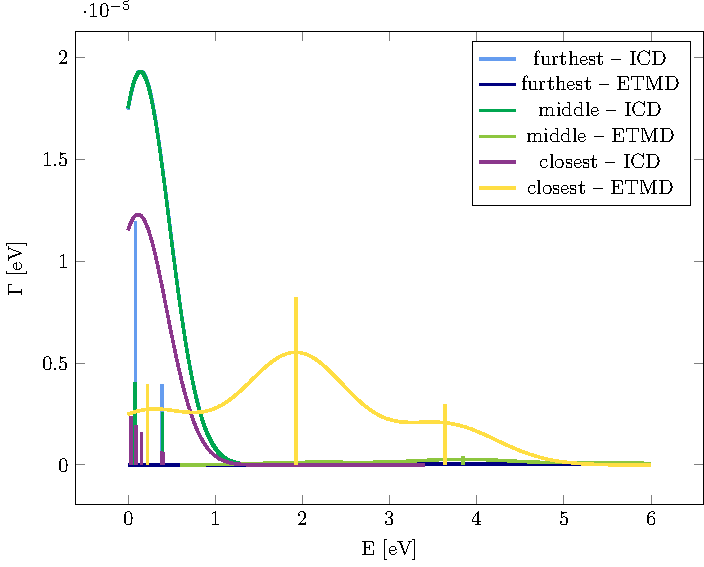
\includegraphics[width=8.5cm]{pics/2tops.pdf}
 \caption{Simulated coincidence spectra of argon clusters consisting of 13
          argon atoms with 2 additional xenon atoms on top of two different
          argon surfaces. The ICD and ETMD spectra are shown for all three
          different relative positionings of the two xenon atoms. In case of
          the two xenon atoms being close to each other, an ETMD process is
          clearly visible. In the other two cases the spectra are dominated by
          the corresponding ICD spectrum.}
 \label{figure:2tops}
\end{figure}

In all three cases both ICD and ETMD(3) are energetically allowed and the ICD
spectra are either identical or at least very similar consisting of one
convoluted peak at approximately \unit[0.2]{eV}. However, the ETMD(3) spectra
are very sensitive to the relative positioning of the two xenon atoms.
Two aspects have to be taken into account: an energy shift of the peak due
to different charge distances in the final state (i.e. the interatomic Xe-Xe
distance) and the different decay widths decreasing with $\frac{1}{R^6}$
between the electron transfer unit and the finally ionized xenon atom.
The larger the distance between the xenon atoms is, the lower are the energies
of the secondary electrons and the higher are the decay widths. Therefore a
significant contribution from the ETMD(3) compared to the ICD is only
to be seen in case of the two xenon atoms residing on two adjacent
surfaces. The threefold peak structure of the ETMD(3) peak does in contrast to
the ICD spectrum not stem from different triple structures but from the
four different decay channels for one triple structure.


For the 55 atoms clusters the xenon content of \unit[10--12]{\%}
corresponds to six xenon atoms out of the 55 total atoms. These can have
different relative positions in the cluster. They could either be grouped
together in one part of the cluster or be evenly distributed in the cluster
as shown in Figure \ref{figure:cluster_3_overview} Panels b) and c). Their
ICD and ETMD(3) spectra are shown in Figure \ref{figure:ar_3_6in}.

\begin{figure}[h]
 \centering
 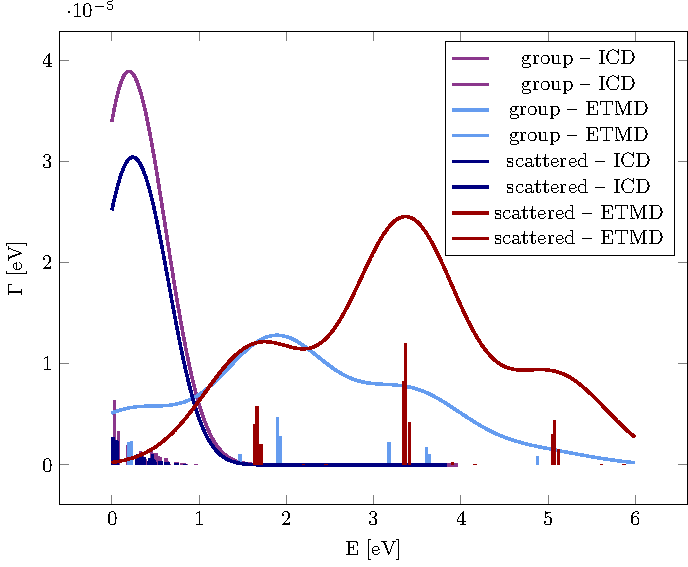
\includegraphics[width=8.5cm]{pics/ar_3_6in.pdf}
 \caption{Simulated ICD and ETMD electron spectra for clusters consisting of
          55 atoms out of which 6 are xenon atoms. These are either clustered
          (group) on one side of the cluster of evenly distributed
          inside the cluster (scattered). In both cases the ETMD peaks are
          clearly visible in the spectra.}
 \label{figure:ar_3_6in}
\end{figure}

For both cases the overall ICD spectra are very similar with concoluted
peaks at approximately \unit[0.3]{eV}. For the grouped xenon atoms ICD
signals at slightly higher energies are to be observed from ArXe pairs of
larger distances du to the different cluster structure. However, the
significant difference is to be observed in the ETMD(3) spectra. The
interatomic xenon distance in the grouped xenon is shorther than in the
cluster with evenly distributed xenon atoms. Hence, the threefold
peak structure for the cluster with the grouped xenon atoms is seen at
lower ETMD(3) electron energies than for the cluster with evenly
distributed xenon atoms. Additionally, the probabilty for an electron
transfer from a xenon to an argon atom decreases exponentially with the
interatomic distance. Therefore, only those xenon atoms which have argon
atoms as their direct neighbours have a significant contribution to the
total decay width and the total ETMD(3) decay width for the structure with
the grouped xenon atoms is lower than the total ETMD(3) decay width of
the structure with evenly distributed xenon atoms.


For comparison with the previous assumptions of a xenon core surrounded
by argon atoms we investigated 13 and 55 atoms clusters with one or two
xenon atoms in the core. Some of the corresponding
spectra are shown in Figure \ref{figure:xe_3_in}.

\begin{figure}[h]
 \centering
 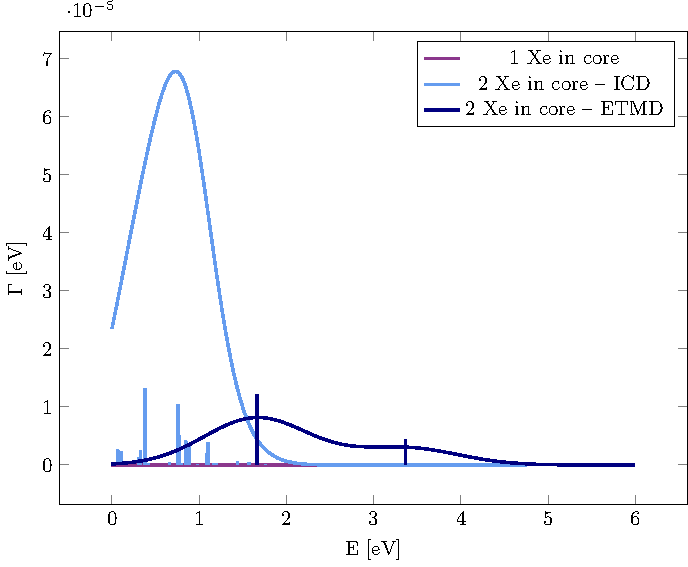
\includegraphics[width=8.5cm]{pics/xe_3_in.pdf}
 \caption{Simulated ICD and ETMD electron spectra for argon clusters with
          one or two atoms in the core of the cluster. In case of the xenon
          atom inhabiting the central position of the cluster for a 13 atoms
          cluster (not shown here) and a 55 atoms cluster all channels are closed
          for all pairs, which leads to no signal. For those clusters with two
          xenon atoms in the core the first ICD channel is open for some pairs
          and additionally ETMD is possible for multiple triples. Due to a
          different distance distribution compared to the clusters with an argon
          core the ICD peak is shifted to higher kinetic energies.}
 \label{figure:xe_3_in}
\end{figure}

For the clusters with only one xenon atom in the core and the ionization
energies used for the simulation of the secondary electron energies
all ICD channels are closed. Since the cluster contains only one xenon atom,
an ETMD(3) is not possible. Hence there is no signal to be expected at all.
For a core consisting of two xenon atoms both an ICD and an ETMD(3) spectrum
can be seen. Compared to the argon core cluster structures the ICD peak is
shifted to higher ICD electron energies not being in agreement with
the experimental spectrum. Additionally, the ICD and ETMD(3) spectra overlap.
In case of the ETMD(3) only three of the four different decay channels are
anergetically allowed.


Originally, very large argon-xenon clusters were measured experimentally,
which we approximate by a cluster consisting of 1415 xenon atoms surrounded
by two complete layers of argon atoms. The spectra are shown in Figure
\ref{figure:xe_8_lay1}.

\begin{figure}[h]
 \centering
 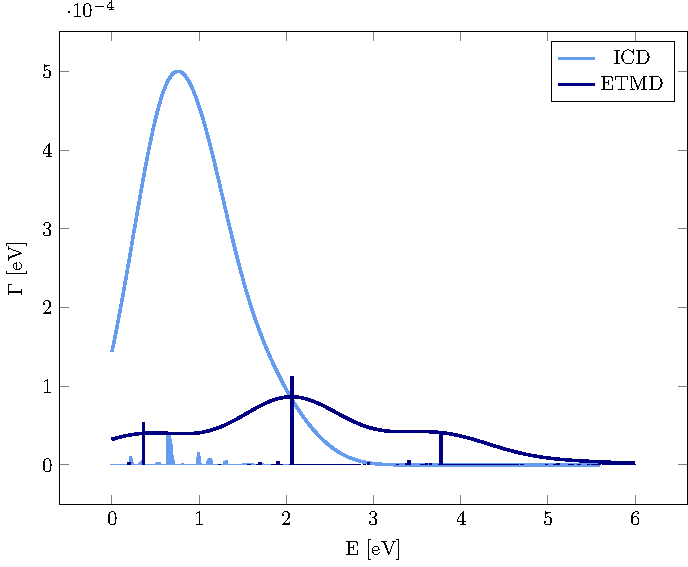
\includegraphics[width=8.5cm]{pics/xe_8_1lay.pdf}
 \caption{Simulated ICD and ETMD electron spectra for a large cluster consisting
          of a xenon core of 1415 atoms surrounded by two complete layers of
          argon atoms. The ICD and ETMD peak overlap such, that the peak structure
          might not be visible.}
 \label{figure:xe_8_lay1}
\end{figure}

Compared to the small clusters with a xenon core in Figure \ref{figure:xe_3_in}
the ICD peak is broadened and shifted to higher ICD electron energies which could be
expected due to the larger interatomic Ar-Xe distances in the large cluster and
the better stabilization of charges (the final state), which was taken care of
in the input of the simulation.
The ETMD(3) peak is as well shifted to slightly higher energies allowing for the
fourth decay channel to open.
